\documentclass[12pt]{beamer}

\usepackage{graphicx,url}
\usepackage[brazil]{babel}
\usepackage[utf8]{inputenc}
\usepackage{mathtools}
\usepackage{fix-cm}
\usepackage{eucal}
\usepackage{amscd}
\usepackage{amsmath}
\usepackage{amssymb}
\usepackage{listings}
\usepackage{colortbl}
\usepackage{latexsym}
\usepackage{verbatim}
\usepackage{hyperref}

\usetheme{Dresden}
\usecolortheme{beaver}
\setbeamertemplate{navigation symbols}{}

\title[Gráficos de Controle]{Gráficos de Controle}

\author{Ramon Santos Nascimento}

\institute[UFRPE]{
  \centering 
\includegraphics[width=1.6cm]{img/logo.png}\\

  \medskip
  Universidade Federal Rural de Pernambuco \\
  \medskip

  \textit{ramonsantos.dev@gmail.com}
}

\date{18 de Junho de 2015}

\subject{Gráficos de Controle}

\begin{document}
  \frame{\titlepage}

  \begin{frame}[t]{Agenda}
    \begin{itemize}
      \item Introdução\newline

      \item Gráficos de Controle\newline

      \item Tipos de Gráficos de Controle\newline

      \item Ferramentas de Apoio\newline

      \item Referências
    \end{itemize}
  \end{frame}

%

  \section{Introdução}
  \label{sec:intro}

  \begin{frame}[t]{O que é Controle Estatístico de Processo?}
    \begin{block}{Definição}
      \emph{O \textbf{Controle Estatístico do Processo (CEP)} é uma técnica estatística que envolve a coleta, a organização e a interpretação de dados para o controle de um processo de produção(ou serviço), com o objetivo de controlar e melhorar continuamente a qualidade do produto.}
    \end{block}
  \end{frame}

  \begin{frame}[t]{Um Breve Histórico Sobre CEP}
    \begin{block}{Década de 20}
      Em 1924 o Dr. Walter A. Shewhart escreveu um memorando mostrando um moderno gráfico(carta) de controle. Harold F. Dodge e Harry G. Roming trabalharam no desenvolvimento da amostragem com base estatística e métodos de inspeção.
    \end{block}

    \begin{block}{Segunda Guerra Mundial}
      O CEP foi usando largamente na industria estadunidense como parte importante no esforço de guerra.
    \end{block}

    \begin{block}{Pós-guerra}
      Os japoneses aplicam CEP em sua industria, e já na década de 70, abrem vantagem competitiva.
    \end{block}
  \end{frame}

  \begin{frame}[t]{Onde é possível aplicar CEP?}
    \begin{itemize}
      \item Planejamento e Desenvolvimento de Produtos;

      \item Determinar Capacidade de um Processo de Fabricação;

      \item Investigar Melhorias no Processo;

      \item Fornecer Confiabilidade e outros Dados de Desempenho de Produtos ou Serviços.
    \end{itemize}
  \end{frame}

  \begin{frame}[t]{Ferramentas importantes de CEP}
    \begin{itemize}
      \item Histograma;

      \item Gráfico de Pareto;

      \item Diagrama de causa-e-efeito;

      \item Diagrama de concentração de defeito;

      \item Diagrama de dispersão;

      \item Folha de verificação;

      \item \textbf{Gráfico de controle.}
    \end{itemize}
  \end{frame}

  \begin{frame}[t]{Histograma}
    \begin{block}{Definição}
      Um histograma é a representação gráfica, em colunas, de um conjunto de dados previamente tabulado e dividido em classes uniformes.
    \end{block}
  \end{frame}

  \begin{frame}{Histograma}
    \begin{figure}[ht]
      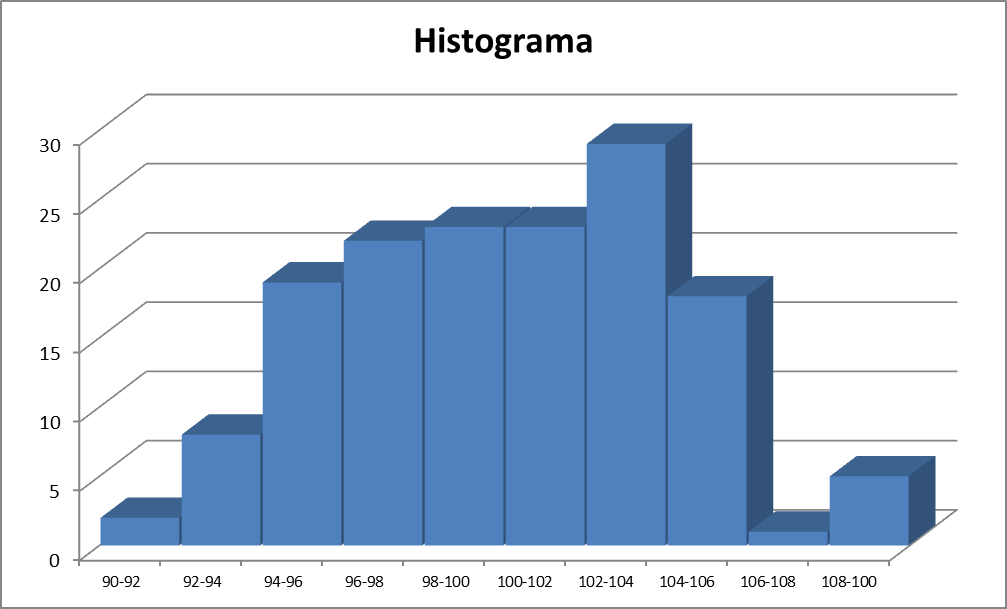
\includegraphics[width=0.7\textwidth]{img/histograma-industria}
      \caption{Histograma}
    \end{figure}
  \end{frame}

  \begin{frame}[t]{Gráfico de Pareto}
    \begin{block}{Definição}
      O diagrama de Pareto é um gráfico de colunas que ordena as frequências das ocorrências, da maior para a menor, permitindo uma fácil visualização e identificação dos problemas mais importantes, possibilitando a concentração de esforços sobre os mesmos.
    \end{block}

    \begin{block}{Obs.}
      Deriva do Princípio de Pareto(80/20).
    \end{block}
  \end{frame}

  \begin{frame}{Gráfico de Pareto}
    \begin{figure}[ht]
      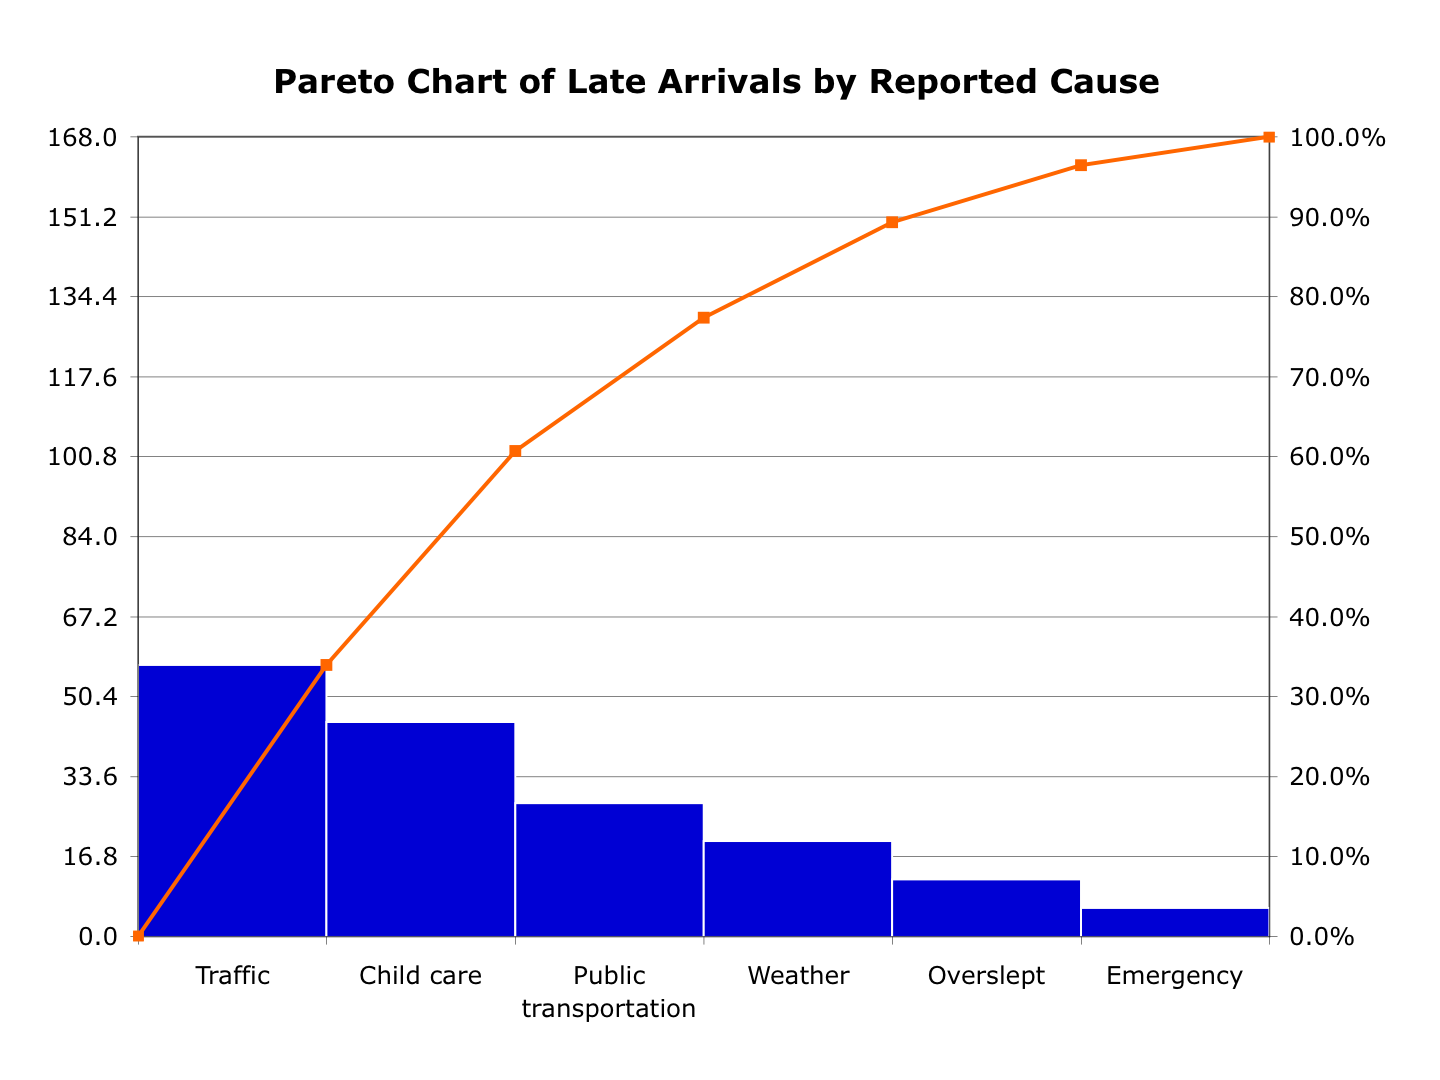
\includegraphics[width=0.6\textwidth]{img/diag-pareto}
      \caption{Gráfico de Pareto}
    \end{figure}
  \end{frame}

%

  \section{Gráficos de Controle}

  \begin{frame}[t]{Causas Casuais}
    \begin{itemize}
      \item Em qualquer processo de produção, uma certa quantidade de variabilidade(ou ruído de fundo) natural sempre existirá. Esse ruído é o efeito cumulativo de muitas causas pequenas, essencialmente inevitáveis.

      \item Um processo que esteja operando apenas com causas casuais de variação presente é dito estar \emph{sob controle estatístico}.
    \end{itemize}
  \end{frame}

  \begin{frame}[t]{Causas Atribuídas}
    \begin{itemize}
      \item Outros tipos de variabilidade podem ocasionalmente estar presentes na saída de um processo. Essa variabilidade nas características-chave da qualidade geralmente aparecem de três fontes:

      \begin{itemize}
        \item máquinas não propriamente ajustadas;

        \item erros dos operadores;

        \item matérias-primas defeituosas.
      \end{itemize}

      \item Tal variabilidade é geralmente grande quando comparada ao ruído de fundo, representando usualmente um nível inaceitável de desempenho de processo.
    \end{itemize}
  \end{frame}

  \begin{frame}[t]{Objetivos dos Gráficos de Controle}
    \begin{itemize}
      \item Um importante objetivo do CEP é detectar a ocorrência de \emph{causas atribuídas} no processo, de modo que uma \emph{investigação do processo} e uma \emph{ação corretiva} possam ser executadas antes que muitas unidades não-conformes sejam fabricadas;

      \item O gráfico de controle é uma técnica de monitoração em tempo real do processo, largamente usada para essa finalidade.
    \end{itemize}
  \end{frame}

  \begin{frame}[t]{Sobre o Gráfico de Controle}
    \begin{itemize}
      \item É uma disposição gráfica de uma característica da qualidade;

      \item Atualizado em intervalos regulares de tempo;

      \item A linha horizontal central representa o valor médio da característica(LC);

      \item A linha horizontal superior representa o valor máximo da característica(LSC);

      \item A linha horizontal inferior representa o valor mínimo da característica(LIC).
    \end{itemize}
  \end{frame}

  \begin{frame}{Sobre o Gráfico de Controle}
    \begin{figure}[ht]
      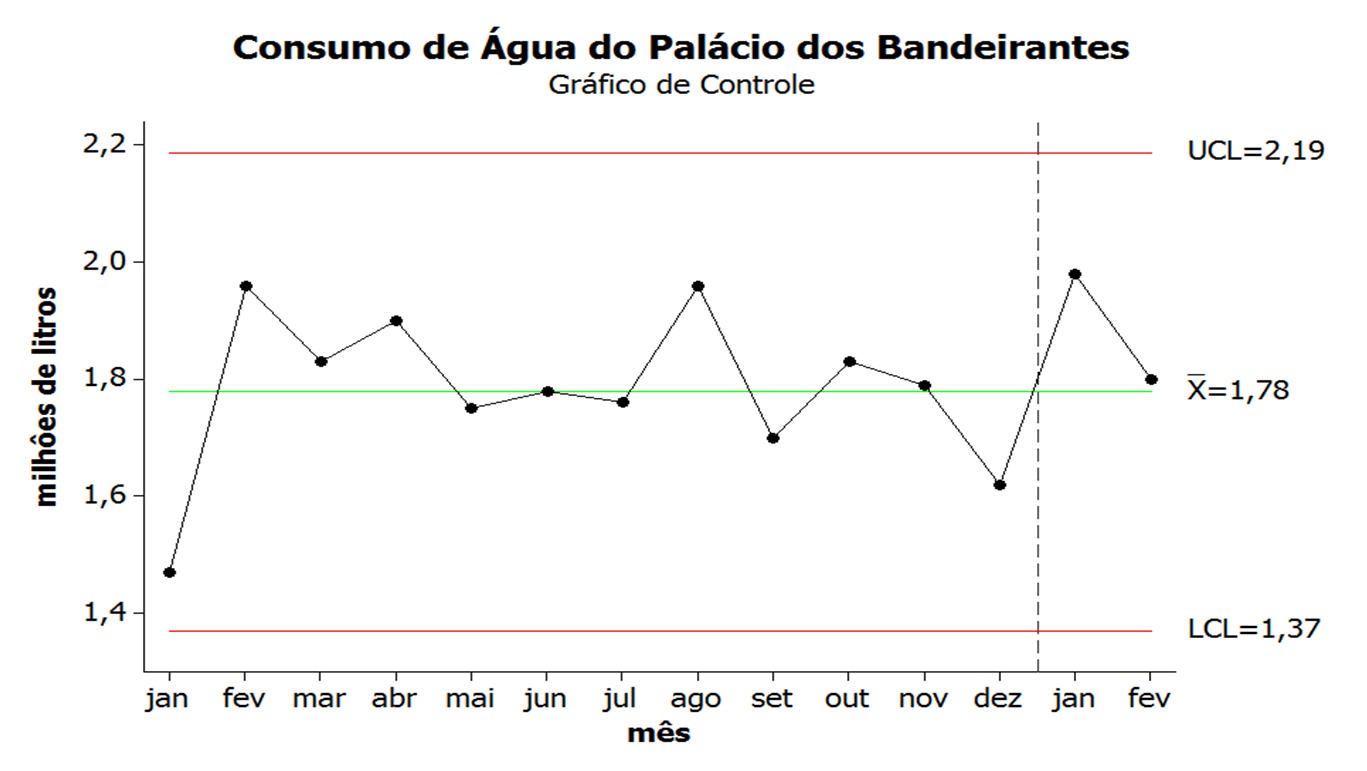
\includegraphics[width=0.7\textwidth]{img/grafico_de_controle_tipico}
      \caption{Gráfico de Controle Típico}
    \end{figure}
  \end{frame}

  \begin{frame}[t]{Sobre o Gráfico de Controle}
    \begin{itemize}
      \item Se todos os pontos estão dentro dos limites de controle mas estão dispostos de forma não aleatória, isso é uma indicação de que o processo está fora de controle;

      \item Essencialmente, o gráfico de controle é um teste de hipótese de que o processo está em um estado de controle estatístico.
    \end{itemize}
  \end{frame}

  \begin{frame}[t]{Modelo de Gráfico de Controle}
    Seja $W$ uma estatística da amostra que mede uma característica de qualidade e suponha que a média seja $\mu_w$ e o desvio-padrão seja $\sigma_w$, temos:

    \begin{align*}
      LSC & =  \mu_{w} + k\sigma_{w} \\
      LC  & =  \mu_w \\
      LIC & =  \mu_w - k\sigma_w
    \end{align*}

    onde $k$ é a distância dos limites de controle a partir da linha central(geralmente $k = 3$), expressa em unidade de desvio-padrão.
  \end{frame}

  \begin{frame}[t]{Popularidade dos Gráficos de Controle}
    Há, no mínimo, cinco razões para sua popularidade. São elas:

    \begin{itemize}
      \item É uma técnica comprovada para melhoria da produtividade;

      \item São efetivos na prevenção de defeitos;

      \item Previnem ajustes desnecessários no processo;

      \item Fornecem informação sobre diagnósticos;

      \item Fornecem informações sobre a capacidade de processo.
    \end{itemize}
  \end{frame}

  \begin{frame}[t]{Projetando um Gráfico de Controle}
    Na fabricação de anéis de pistão de motores automotivos, o diâmetro interno dos anéis é uma característica de qualidade. O diâmetro médio interno do anel no processo é 74 milímetros e sabe-se que o desvio-padrão do diâmetro do anel é 0,001 milímetros.\newline

    A cada hora, uma amostra aleatória de cinco anéis é retirada, o diâmetro médio ($\bar x$) do anel da amostra é calculado e plotado.
  \end{frame}

  \begin{frame}[t]{Projetando um Gráfico de Controle}
    O próximo passo é determinar os limites:

    \begin{align*}
      \sigma_{\bar{X}} = \frac{\sigma}{\sqrt{n}} = \frac{0,001}{\sqrt{5}} = 0,0045
    \end{align*}

    Usando o teorema do limite central para considerar que $\bar X $ seja distribuído de forma aproximadamente normal, espera-se que, aproximadamente, 100(1 - $\alpha$)\% dos diâmetros médios $\bar X  $ das amostras caíssem entre 74 + $z_{\alpha/2}$(0,0045) e 74 - $z_{\alpha/2}$(0,0045).
  \end{frame}

  \begin{frame}[t]{Projetando um Gráfico de Controle}
    Um valor padrão para $z_{\alpha/2}$ é 3, então temos:

    \begin{align*}
      LSC & =  74 + 3x(0,0045) = 74,0135 \\
      LIC & =  74 - 3x(0,0045) = 73,9865
    \end{align*}
  \end{frame}

%

  \section{Tipos de Gráficos de Controle}

  \begin{frame}[t]{Tipos de Gráficos de Controle}
    \begin{itemize}
      \item $\bar X$ e R;

      \item $\bar X$ e S;

      \item CUSUM;

      \item EWMA.
    \end{itemize}
  \end{frame}

  \begin{frame}[t]{Tipos de Gráficos de Controle}
    Quando lidando com uma característica de qualidade que pode ser expressa como uma medida, é comum monitorar tanto o valor médio quanto sua variabilidade.\newline

    Pode-se usar o gráfico $\bar X$ com o $R$(Amplitude) ou o $\bar X$ com o $S$(Desvio-Padrão).
  \end{frame}

  % XR

  \begin{frame}[t]{Gráficos $\bar X$ e R}
    \begin{itemize}
      \item \textbf{$\bar X$ e R;}

      \item $\bar X$ e S;

      \item CUSUM;

      \item EWMA.
    \end{itemize}
  \end{frame}

  \begin{frame}[t]{Gráficos $\bar X$ e R}
    \begin{itemize}
      \item Amplitude e Média;

      \item Baseado na Distribuição Normal;

      \item Indicado quando o tamanho da amostra é constante e relativamente pequeno(menor que 10).
    \end{itemize}
  \end{frame}

  \begin{frame}[t]{Gráficos $\bar X$ e R}
    A linha central e os limites superior e inferior de controle para o gráfico de controle $\bar X$ são

    \begin{align*}
      LSC & = \bar{\bar x} + A_{2}{\bar{r}}\\
      LC & = \bar{\bar x}\\
      LIC & = \bar{\bar x} - A_{2}{\bar{r}}
    \end{align*}

    onde $\bar{r}$ é a aplitude média e a constante $A_{2}$ é tabelada, para vários tamanhos de amostra.
  \end{frame}

  \begin{frame}{Gráficos $\bar X$ e R}
    \begin{figure}[c]
      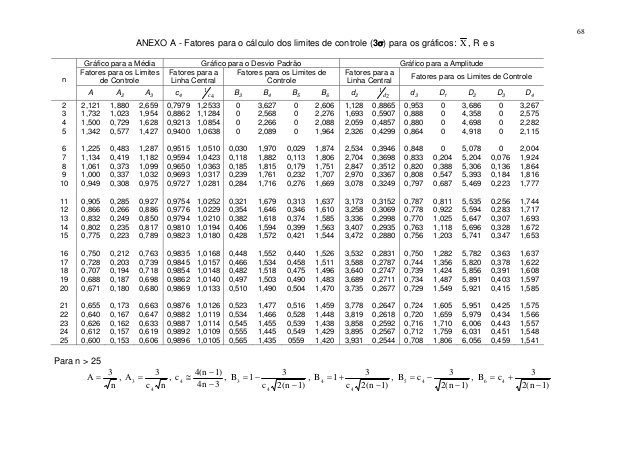
\includegraphics[width=0.75\textwidth]{img/tabela-r}
      \caption{Fatores para a Construção do Gráficos}
    \end{figure}
  \end{frame}

  \begin{frame}[t]{Gráficos $\bar X$ e R}
    A linha central e os limites superior e inferior de controle para o gráfico de controle $R$ são

    \begin{align*}
        LSC & = D_4 \bar r\\
        LC & = \bar r\\
        LIC & = D_3 \bar r
    \end{align*}

    onde $\bar r$ é amplitude média da amostra e as constantes $D_3$ e $D_4$ também são tabeladas.
  \end{frame}

  \begin{frame}[t]{Exemplo $\bar X$ e R}
    \begin{figure}[ht]
      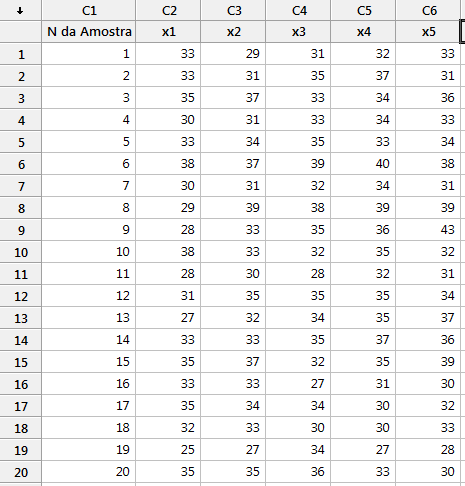
\includegraphics[width=0.45\textwidth]{img/Tabela}
      \caption{Entradas de dados}
    \end{figure}
  \end{frame}

  \begin{frame}[t]{Exemplo $\bar X$ e R}
    \begin{figure}[ht]
      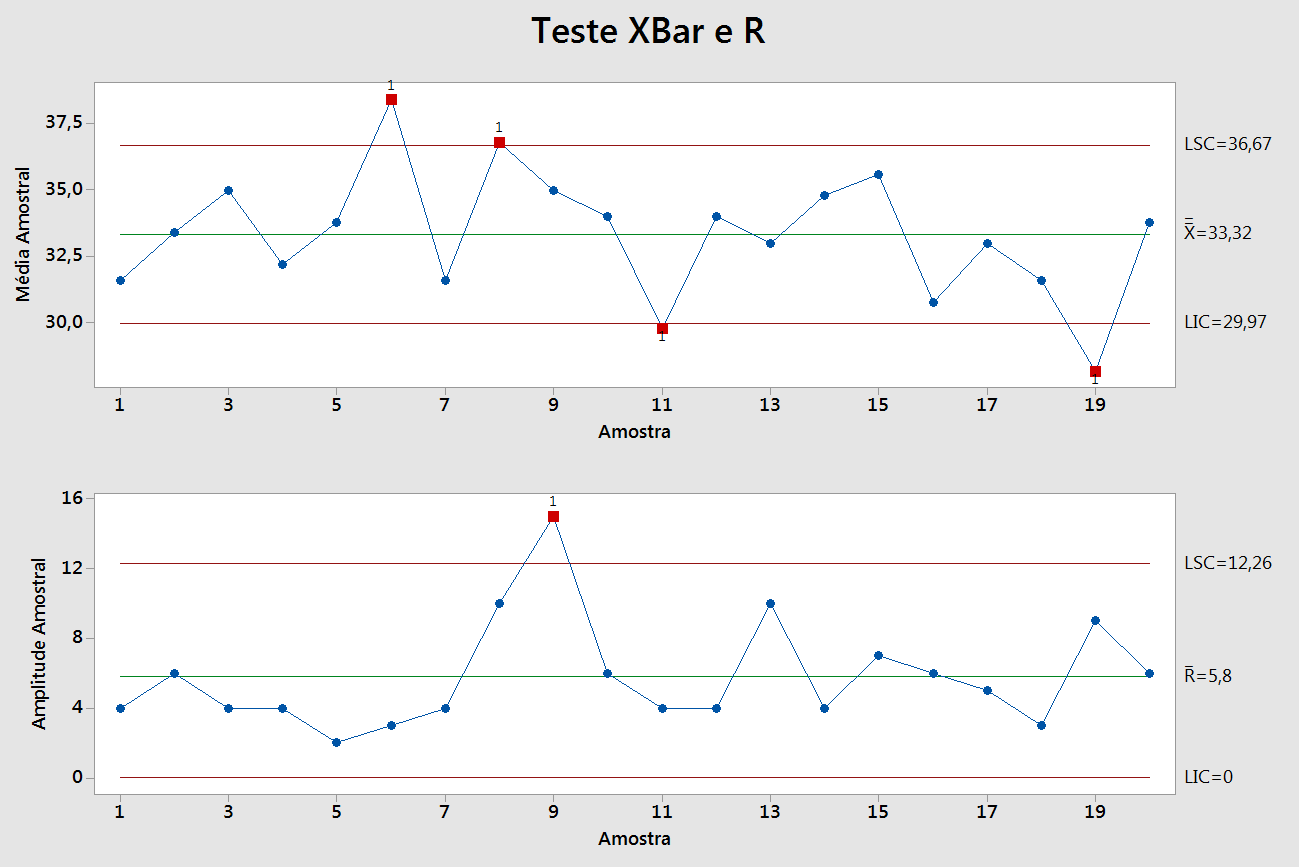
\includegraphics[width=0.7\textwidth]{img/testeR}
      \caption{Gráfico $\bar X$ e R}
    \end{figure}
  \end{frame}

  %XS

  \begin{frame}[t]{Gráficos $\bar X$ e S}
    \begin{itemize}
      \item $\bar X$ e R;

      \item \textbf{$\bar X$ e S;}

      \item CUSUM;

      \item EWMA.
    \end{itemize}
  \end{frame}

  \begin{frame}[t]{Gráficos $\bar X$ e S}
    EM vez de se basear em gráficos de controle para amplitudes, uma abordagem mais moderna é calcular o desvio-padrão de cada subgrupo e plotar esses desvios-padrão para monitorar o desvio-padrão $\sigma$ do processo.
  \end{frame}

  \begin{frame}[t]{Gráficos $\bar X$ e S}
    \begin{itemize}
      \item Desvio-Padrão e Média;

      \item Baseado na Distribuição Normal;

      \item Indicado quando o tamanho da amostra é variável e relativamente grande(maior que 10);

      \item É recomendado o uso de computador para fazer os cálculos.
    \end{itemize}
  \end{frame}

  \begin{frame}[t]{Gráficos $\bar X$ e S}
    A linha central e os limites superior e inferior de controle para o gráfico de controle $\bar X$ são

    \begin{align*}
      LSC & = \bar{\bar x} + A_{3}{\bar{s}}\\
      LC & = \bar{\bar x}\\
      LIC & = \bar{\bar x} - A_{3}{\bar{s}}
    \end{align*}

    onde a constante $A_{3}$ é tabelada, para vários tamanhos de amostra.
  \end{frame}

  \begin{frame}[t]{Gráficos $\bar X$ e S}
    A linha central e os limites superior e inferior de controle para o gráfico de controle $S$ são

    \begin{align*}
      LSC & = D_4 \bar s\\
      LC & = \bar s\\
      LIC & = D_3 \bar s
    \end{align*}

    onde as constantes $D_3 \bar r$ e $D_4 \bar r$ são tabeladas.
  \end{frame}

  \begin{frame}[t]{Exemplo $\bar X$ e S}
    \begin{figure}[ht]
      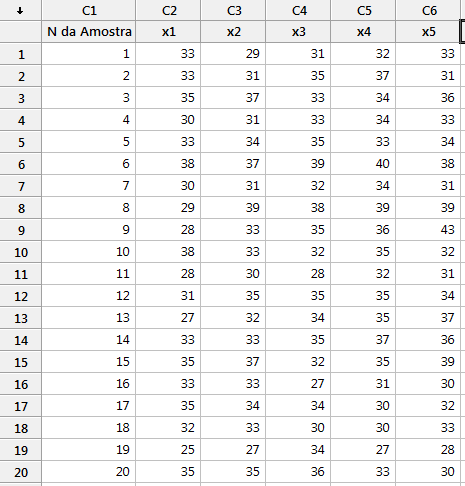
\includegraphics[width=0.45\textwidth]{img/Tabela}
      \caption{Entradas de dados}
    \end{figure}
  \end{frame}

  \begin{frame}[t]{Exemplo $\bar X$ e S}
    \begin{figure}[ht]
      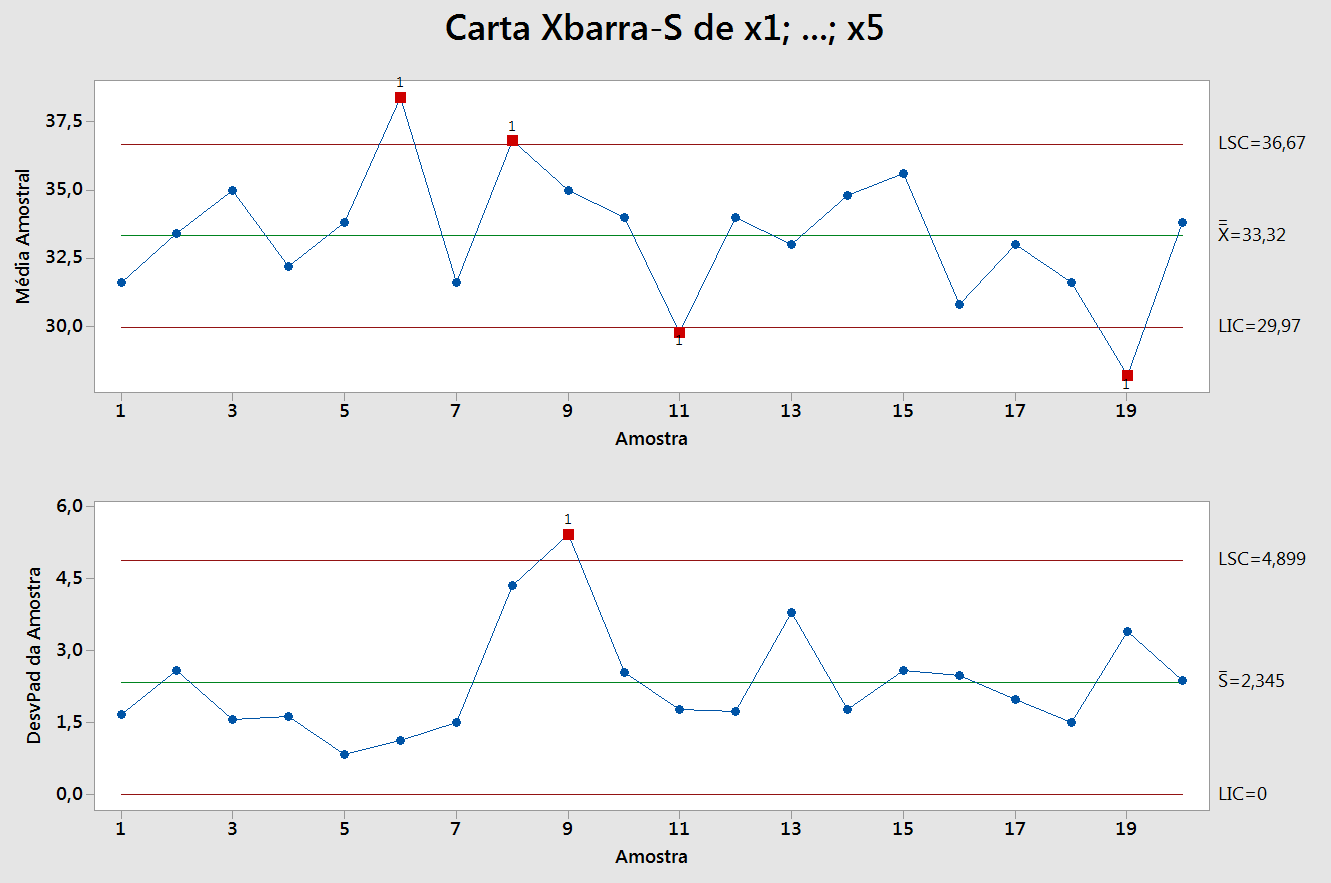
\includegraphics[width=0.7\textwidth]{img/TesteS}
      \caption{Gráfico $\bar X$ e S}
    \end{figure}
  \end{frame}

  % CUSUM

  \begin{frame}[t]{Gráfico de Controle para Soma Cumulativa}
    \begin{itemize}
      \item $\bar X$ e R;

      \item $\bar X$ e S;

      \item \textbf{CUSUM};

      \item EWMA.
    \end{itemize}
  \end{frame}

  \begin{frame}[t]{Gráfico de Controle para Soma Cumulativa}
    \begin{itemize}
      \item Uma grande desvantagem dos gráficos anteriores é que o gráfico é relativamente insensível a pequenas mudanças no processo(algo da ordem de 1,5$\sigma$ ou menos);

      \item A razão disso é que os modelos anteriores usam somente informações no último ponto plotado;

      \item Os gráficos CUSUM são particularmente efetivos com amostras de tamanho 1~(como na industria química e de processos).
    \end{itemize}
  \end{frame}

  \begin{frame}[t]{Gráfico de Controle para Soma Cumulativa}
    O gráfico CUSUM plota as somas cumulativas dos desvios dos valores amostrais em relação ao valor-alvo

    \begin{align*}
      S_i & = \sum_{j=1}^{i} (\bar{X_{j}} - \mu_{0})
    \end{align*}

    onde $\mu_0$ é o alvo da média do processo e $\bar{X_{j}}$ é a média da j-ésima.
  \end{frame}

  \begin{frame}[t]{Gráfico de Controle para Soma Cumulativa}
    \begin{itemize}
    \item Se o processo permanecer sob controle no valor alvo $\mu_0$, a soma cumulativa definida na equação anterior deve flutuar em torno de zero;

    \item Consequentemente, se uma tendência se desenvolver nos pontos plotados para cima ou para baixo, deve-se considerar isso como uma evidência de causa atribuída.
    \end{itemize}
  \end{frame}

  \begin{frame}[t]{Limites no CUSUM}
    Há duas abordagens gerais para imaginar limites de controle para CUSUMs:

    \begin{itemize}
      \item Máscara em $V$;

      \item CUSUM Tabular.
    \end{itemize}
  \end{frame}

  \begin{frame}[t]{Máscara em V}
    Máscara em $V$ é um entalhe em forma de $V$ em um plano que pode ser colocado em diferentes localizações em um gráfico.

    \begin{figure}[ht]
      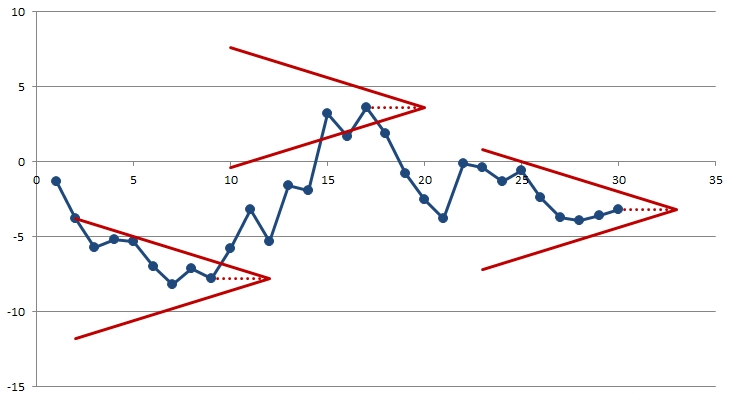
\includegraphics[width=0.7\textwidth]{img/grafico_CUSUM_mask_v}
      \caption{Exemplo da Máscara em V}
    \end{figure}
  \end{frame}

  \begin{frame}[t]{CUSUM Tabular}
    Seja $S_H(i)$ um CUSUM unilateral superior e $S_L(i)$ um CUSUM unilateral inferior, ambos para o período i. Essas grandezas são calculadas a partir de

    \begin{align*}
      S_H(i) & = max[0, \bar{X_i} - (\mu_0 + K) + S_H(i - 1)]\\
      S_L(i) & = max[0, (\mu_0 - K) - \bar{X_i} + S_L(i - 1)]\\
           K & = \frac{\Delta}{2} = \frac{|\mu_1 - \mu_0|}{2}
    \end{align*}

    em que os valores iniciais $S_H(0) = S_L(0) = 0$.
  \end{frame}

  \begin{frame}[t]{Exemplo CUSUM}
    \begin{table}[h]
      \centering

      \begin{tabular}{|l|l|l|l|}
        \hline
        102,0 & 98,5  & 101,3 & 96,7  \\ \hline
        94,8  & 99,0  & 98,7  & 101,2 \\ \hline
        98,3  & 97,7  & 101,1 & 101,4 \\ \hline
        98,4  & 100,0 & 98,4  & 102,0 \\ \hline
        102,0 & 98,1  & 97,0  & 102,9 \\ \hline
      \end{tabular}

      \caption{Amostras}
    \end{table}

    Onde cada célula representa uma amostra(de cima para baixo e da esquerda para a direita).
  \end{frame}

  \begin{frame}[t]{Exemplo CUSUM}
    \begin{figure}[ht]
      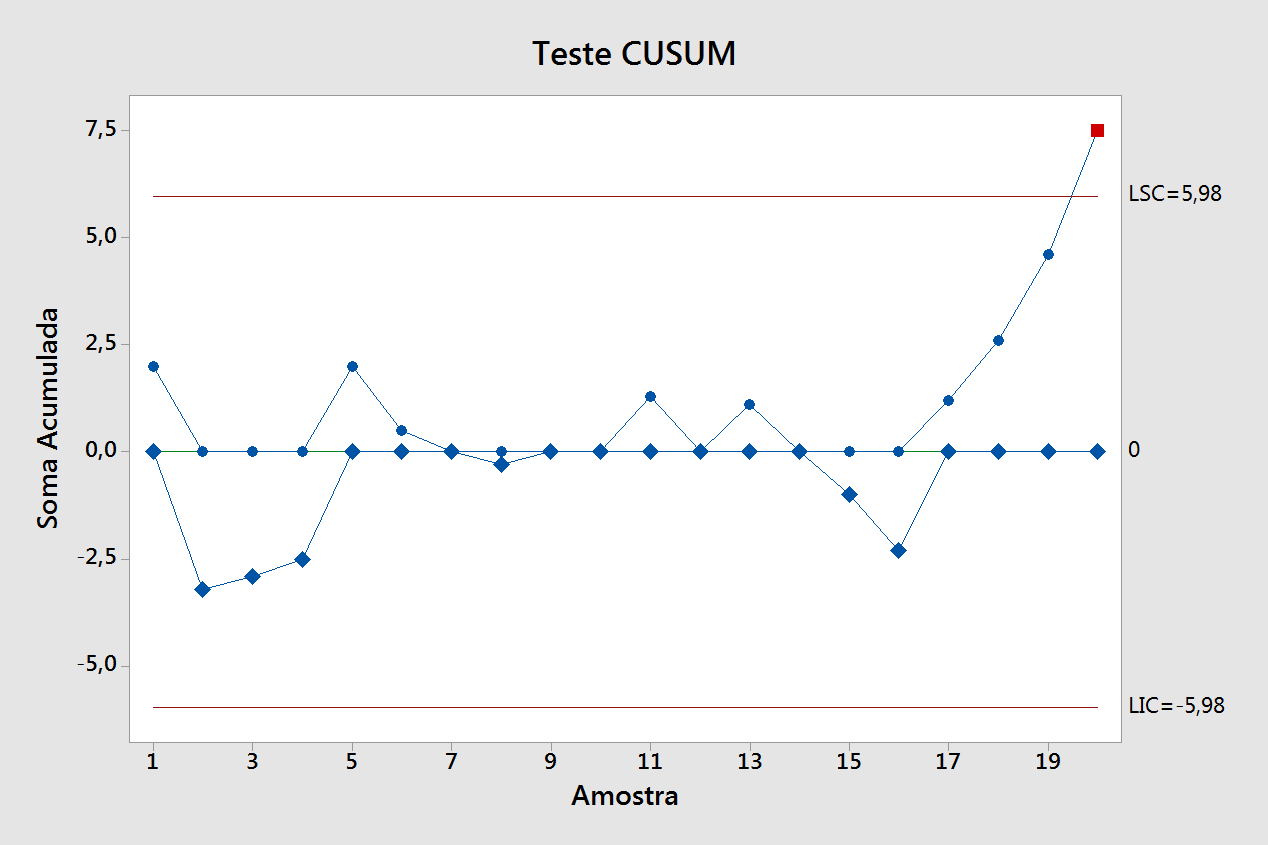
\includegraphics[width=0.7\textwidth]{img/teste_cusum}
      \caption{Gráfico CUSUM}
    \end{figure}
  \end{frame}

  \begin{frame}[t]{Média Móvel Ponderada Exponencialmente}
    \begin{itemize}
      \item $\bar X$ e R;

      \item $\bar X$ e S;

      \item CUSUM;

      \item \textbf{EWMA}.
    \end{itemize}
  \end{frame}

  \begin{frame}[t]{Média Móvel Ponderada Exponencialmente}
    \begin{itemize}
      \item EWMA - Exponentially-Weighted Moving Average;

      \item Usa a média dos dados recentes para suavizar o ruído nos dados e gerar uma estimativa melhor;

      \item Os pontos plotados em um gráfico EWMA não são independentes;

      \item $\lambda$ $(0 < \lambda \le 1)$ representa os pesos;

      \item O valor de $\lambda$ é geralmente escolhido a partir da faixa $(0,1 < \lambda < 0,5)$.
    \end{itemize}
  \end{frame}

  \begin{frame}[t]{Média Móvel Ponderada Exponencialmente}
    A equação de atualização de EWMA é dada por

    \begin{align*}
      Z_t = \lambda \bar{X_t} + (1 - \lambda)Z_t - 1
    \end{align*}
  \end{frame}

  \begin{frame}[t]{Média Móvel Ponderada Exponencialmente}
    Os limites são colocados a três desvios-padrão em torno da médio da estatística plotada $Z_t$.

    \begin{align*}
      LSC & = \mu_0 + 3\frac{\sigma}{\sqrt{n}}\sqrt{\frac{\lambda}{2 - \lambda}[1 - (1 - \lambda)^{2t}]}\\
      LC  & = \mu_0\\
      LIC & = \mu_0 - 3\frac{\sigma}{\sqrt{n}}\sqrt{\frac{\lambda}{2 - \lambda}[1 - (1 - \lambda)^{2t}]}
    \end{align*}
  \end{frame}

  \begin{frame}[t]{Média Móvel Ponderada Exponencialmente}
    \begin{itemize}
      \item Os limites não são de igual largura em torno da linha central;

      \item Os limites são calculados a partir da variância de $Z_t$ e ela muda com o tempo;

      \item Para $t$ grande, a variância de $Z_t$ converge para
    \end{itemize}

    \begin{align*}
      \lim_{t \to \infty} V(Z_t) = {\frac{\sigma^2}{n}}(\frac{\lambda}{2 - \lambda})
    \end{align*}
  \end{frame}

  \begin{frame}[t]{Exemplo EWMA}
    \begin{table}[h]
      \centering

      \begin{tabular}{|l|l|l|l|}
        \hline
        102,0 & 98,5  & 101,3 & 96,7  \\ \hline
        94,8  & 99,0  & 98,7  & 101,2 \\ \hline
        98,3  & 97,7  & 101,1 & 101,4 \\ \hline
        98,4  & 100,0 & 98,4  & 102,0 \\ \hline
        102,0 & 98,1  & 97,0  & 102,9 \\ \hline
      \end{tabular}

      \caption{Amostras}
    \end{table}

    onde cada célula representa uma amostra(de cima para baixo e da esquerda para a direita)
  \end{frame}

  \begin{frame}[t]{Exemplo EWMA}
    \begin{figure}[ht]
      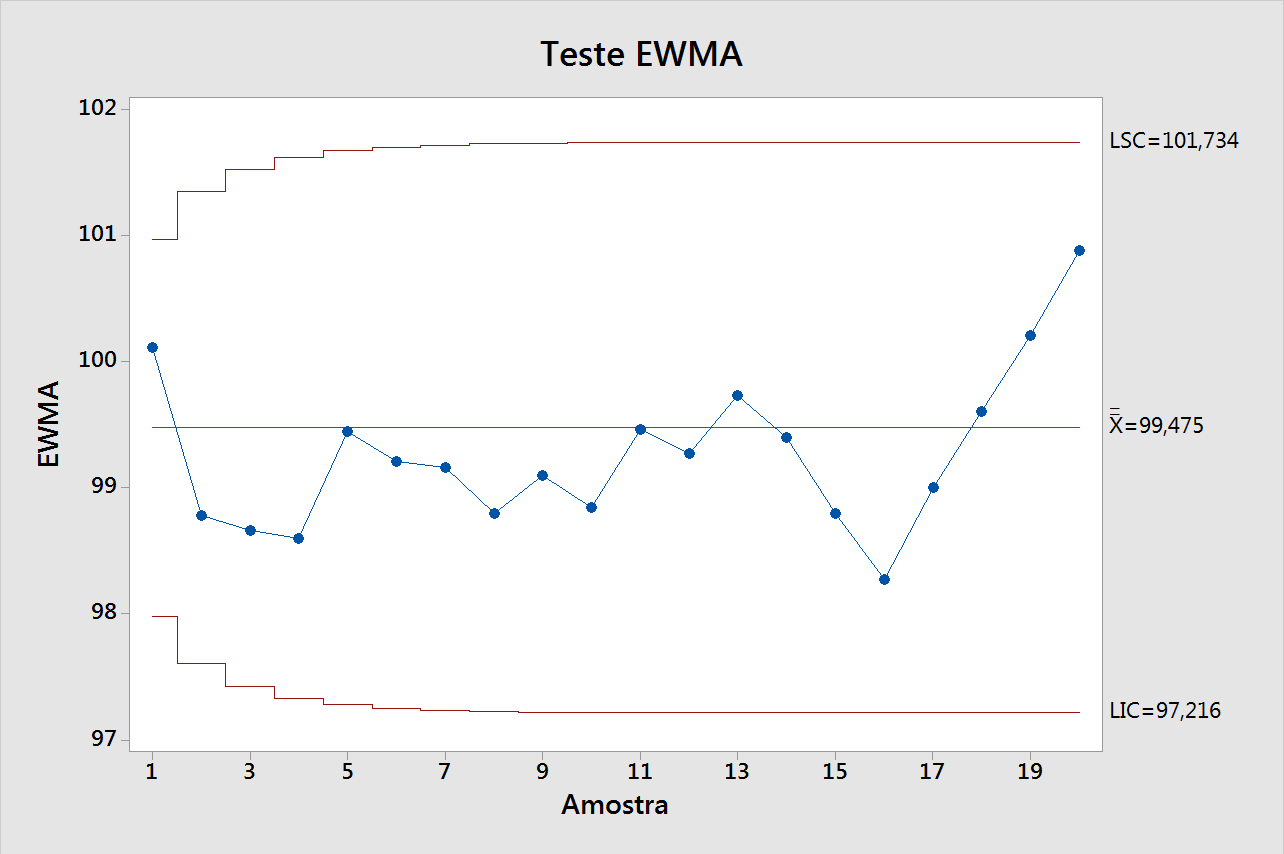
\includegraphics[width=0.7\textwidth]{img/teste_ewma}
      \caption{Gráfico EWMA}
    \end{figure}
  \end{frame}

%

  \section{Ferramentas de Apoio}

  \begin{frame}[t]{Algumas Ferramentas de Apoio}
    \begin{itemize}
      \item Minitab;
        \begin{itemize}
          \item {\url{http://www.minitab.com/pt-br/products/minitab/features/}}
        \end{itemize}

      \item R;
        \begin{itemize}
          \item {\url{http://www.r-project.org/}}

          \item {\url{http://cran.r-project.org/web/packages/qcc/index.html}}

          \item {\url{http://www.rstudio.com/products/rstudio/}}
        \end{itemize}

      \item Microsoft Excel.
        \begin{itemize}
          \item {\url{https://products.office.com/pt-br/excel}}
        \end{itemize}
    \end{itemize}
  \end{frame}

  \begin{frame}[t]{Minitab}
    \begin{figure}[ht]
      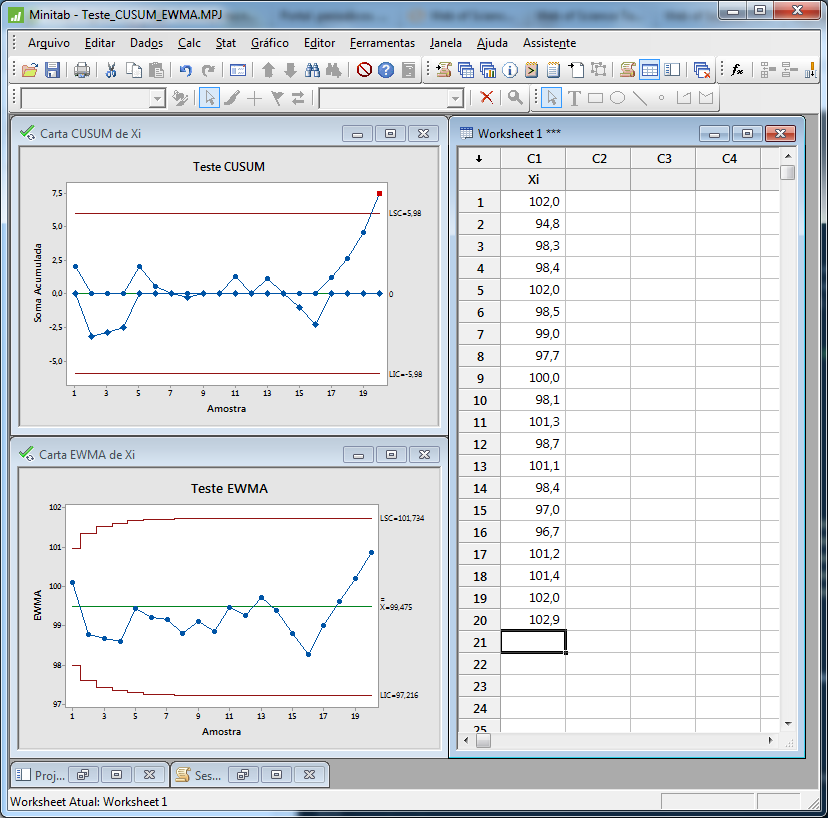
\includegraphics[width=0.5\textwidth]{img/minitab_img}
      \caption{Aspecto do Minitab}
    \end{figure}
  \end{frame}

%

  \section{Referências}

  \begin{frame}[t]
    \frametitle<presentation>{{Referências Bibliográficas}}

    \begin{thebibliography}{10}
      \beamertemplatebookbibitems
        \bibitem{Montgomery}
          Douglas C. Montgomery, George C. Runger
          \newblock {\em Estatística Aplicada e Probabilidade para Engenheiros}.
          \newblock LTC, 2009.

        \bibitem{Levine}
          David Levine, David Stephan, Timothy Krehbiel, Mark Berenson
          \newblock {\em Estatística - Teoria e Aplicações usando o Microsoft Excel}.
          \newblock LTC, 2005.

      \beamertemplatearticlebibitems
        \bibitem{Kappel}
          Mateus Kappel, Aurélia Rodrigues
          \newblock O uso do gráfico de controle $\bar{X}$  e R no monitoramento do volume de envase de refrigerante.
          \newblock {\em FAMAT em Revista}, 10:21--32, 2008.
    \end{thebibliography}
  \end{frame}

%

  \section{}

  \begin{frame}{Dúvidas}
    \Huge{\centerline{Dúvidas?}}
  \end{frame}

  \begin{frame}{Obrigado}
    \Huge{\centerline{Obrigado!}}
  \end{frame}
\end{document}
